\chapter{Related Works}
In this chapter, the topics related to the work of this thesis are introduced and discussed. The topics include mainly three parts: \textbf{Heuristic Negotiation Strategies for Autonomous Negotiation}, \textbf{Reinforcement Learning used in Autonomous Negotiation} and \textbf{Challenges in Deep Reinforcement Learning}. Several time-based, behavior-based and concurrent negotiation methods are discussed in the section heuristic negotiation strategies. The content of the second part is about the \gls{rl} framework used in autonomous negotiation. Finally, some frequently appearing challenges when applying deep reinforcement learning are specified in the section challenges in deep reinforcement learning.

\section{Heuristic Negotiation Strategies for Autonomous Negotiation} \label{related-work:heuristic-negotiation}
\subsection{Time-based Strategy (Aspiration Negotiator)}
Aspirations are the specific goals in a negotiation that a negotiator wishes to achieve as part of an agreement. Empirical evidence has shown that negotiators with higher aspirations tend to achieve better bargaining results.. First, aspiration of negotiator can help to determine the outer limit of what negotiator will request. Second, optimistic aspirations can make the negotiators to work harder\parencite{Schneider2004}. Many aspiration negotiators are time dependent, such as \textbf{Boulware} (with concession factor $e=1/2$), \textbf{Linear} ($e=1$) and \textbf{Conceder} ($e=2$)\parencite{FARATIN1998159}. Boulwarism is the tactic of making a "take-it-or-leave-it" offer in a negotiation, with no further concessions or discussion. It was named after General Electric's former vice president Lemuel Boulware, who promoted the strategy\parencite{William1991}.

At every round, the agent (negotiator) calculates their decision utility which determines whether they accept an offer or not. For time-dependent agent, the utility is:
\begin{equation}
u(t) = P_{min} + (P_{max} - P_{min})(1-\alpha(t))
\end{equation}
$P_{max}$ and $P_{min} \in [0, 1]$ means the minimum utility and the maximum utility, respectively. Frequently, $\alpha(t)$ is parametrized as a time-depedent polynomial function\parencite{chang2020multiissue, FARATIN1998159}: 

\begin{equation}
\alpha(t)=\kappa+\left(1-\kappa\right)\left(\min \left(t, t_{\max }\right) / t_{\max }\right)^{1 / e}
\end{equation}

Where $e$ is the concession factor. For simplicity, $k$ is often set to $0$. Figure \ref{fig:boulware-conceder-combination} diagrams the convexity degree of $\alpha(t)$and utility value $u(t)$ based on the $\alpha(t)$.

\begin{figure}
\centering
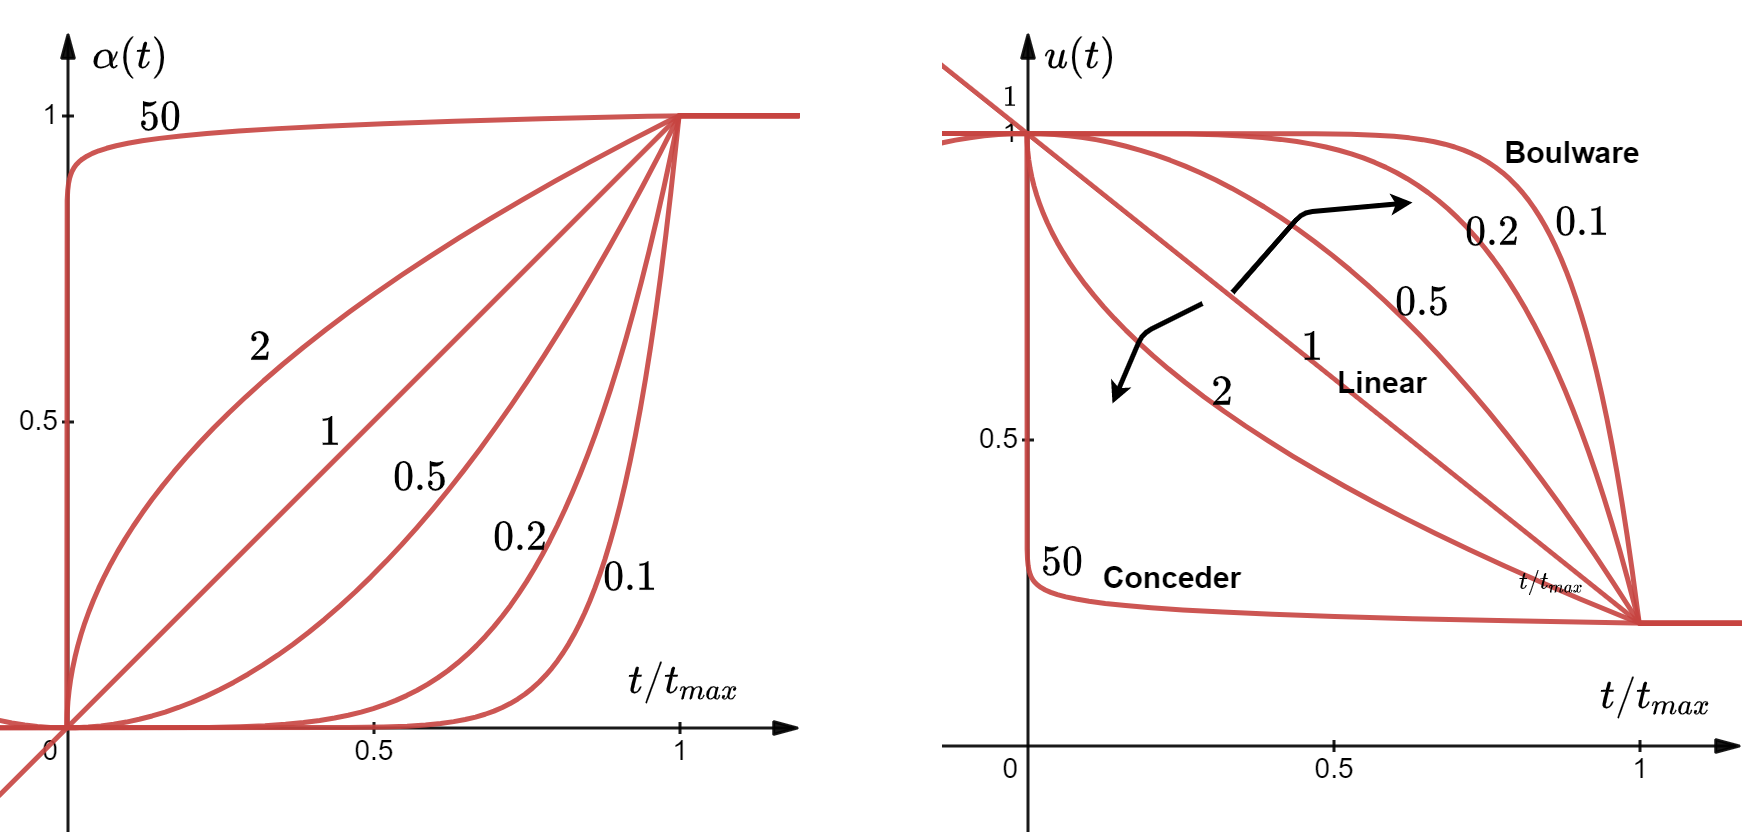
\includegraphics[width=1.0\textwidth]{./images/conceder-boulware-combination.png}
\caption{Convexity degree of $\alpha(t)$ (left) and $u(t)$ (right) with concession factors $e=[0.1, 0.2, 0.5, 1, 2, 50]$.}
\label{fig:boulware-conceder-combination}
\end{figure}

In addition, it is obvious, for single issue, the value of issue $j$ as the offer at time $t$ sent by agent a to agent b can be formed as follows:
\begin{equation}
x_{a \rightarrow b}^{t}[j]=\left\{\begin{array}{ll}
\min _{j}^{a}+\alpha_{j}^{a}(t)\left(\max _{j}^{a}-\min _{j}^{a}\right) & \text { if } u_{j}^{a} \text { is decreasing } \\
\min _{j}^{a}+\left(1-\alpha_{j}^{a}(t)\right)\left(\max _{j}^{a}-\min _{j}^{a}\right) & \text { if } u_{j}^{a} \text { is increasing. }
\end{array}\right.
\end{equation}
Where $u_{j}$ denotes utility value of issue $j$. The minimum and maximum value of issue $j$ are represented by $\min _{j}$ and $\max _{j}$ , respectively.

The offer will always be within the value range ($[min_j, max_j]$), the initial constant will be given at the beginning, and before the deadline is reached, the strategy will suggest an outcome with the reserved value, which is usually the value with minimum utility.

\subsection{Behavior-based Strategies}
Behavior-based and imitation bidding strategies observe the opponent's behavior and decide what to offer and accept. A well-known behavior-based strategy is \textbf{tit-for-tat}. This strategy is to act cooperatively first, and then mirrors what other players did in the previous round.
It is a very robust strategy and has three main following features\parencite{Baarslag2013, chang2020multiissue}:
\begin{itemize}
\item It is never the first to defect (i.e. As long as the opponent also plays well, it will play well).
\item The opponent's defection may lead to retaliation.
\item It can forgive after retaliation.
\end{itemize}
There are two different actions from the opponent that could be considered "nice": The opponent concedes according to its utility function or offers more utility to the agent, according to the agent's utility function. Agent can also choose one of this two options. Therefore, there are four different ways for tit-for-tat agent to reciprocate. When agent reciprocate according to the agent's own utility function and opponent makes a bid that is better for the agent, in return, the agent will produce a bid of lower utility for itself. This is a cooperative behavior. But, agent also considers the utility of its opponent. Bayesian learning is used to construct an opponent model. For nice-tit-for-tat, it uses the opponent model to make an estimate of the location of the Nash point of the negotiation scenario. It uses improved moving ratio to avoid far too nice strategy. For example, if the opponent has made an offer that is 0.7 on the way to the Nash point, the agent will respond in kind by approaching from other side, making an offer that is 0.3 away from the Nash point\parencite{Baarslag2013}. In contrast, if opponent makes a bid that is worse for the agent, in return, the agent will produce a bid of higher utility for itself. It means, opponent is defect, and agent retaliates against the opponent.


\subsection{Concurrent Negotiation Strategy (\gls{cns})}
In a concurrent negotiation environment, an agent will negotiate with many opponents at the same time (one-to-many). One issue is how to coordinate all these negotiations. The author of the paper \parencite{Williams12Concurrent} designed an intuitive model with two key parts, namely the \textbf{Coordinator} and \textbf{Negotiation Thread} to deal with this problem.

\paragraph{Negotiation Threads} The strategy of each negotiation thread is an extension of a principled, adaptive bilateral negotiation agent. This agent was designed to be used in a similarly complex environment, but only for negotiations against a single opponent. In this thread, agent $i$ performs gaussian process regression to predict the future concession of its opponent. With the probability distribution $p_{i, t}(u_i)$ over the utility, prediction of the future concession of opponent can be captured (see \parencite{Williams2011} for details). The probability distribution is then passed to the coordinator.

\paragraph{Coordinator} The role of the coordinator is to calculate the best time $t_i$ to reach agreement and utility value $u_i$ at that time, for each thread. To do so, it uses the probability distribution received from the individual threads, which predict future utilities offered by the opponents.  

Related components and data flow are diagrammed in the figure \ref{fig:heuristic-concurrent-negotiation}.
\begin{figure}[htbp]
\centering
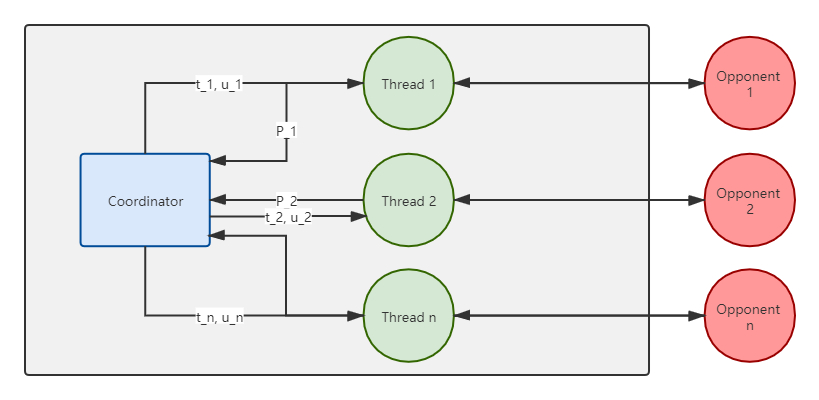
\includegraphics[width=0.8\textwidth]{./images/heuristic_concurrent_negotiation.png}
\caption{Architecture of the concurrent negotiation agent, best time: $t_i$ and utility value: $u_i$, probability distributions: $P$. Own illustration based on\parencite{Williams12Concurrent}.}
\label{fig:heuristic-concurrent-negotiation}
\end{figure}

%\subsection{Optimal Negotiation Strategies}
\subsection{Conclusion}
From the analysis of the heuristic negotiation strategy in automated negotiation, we can extract some important parameters, such as time and the opponent's offer, these parameters can be regarded as important information that affects the negotiation process.

\section{Reinforcement Learning used in Autonomous Negotiation}

\paragraph{\gls{rlboa}} Bak et. al. proposed \parencite{Bakker2019RLBOAAM}, a modular reinforcement learning framework for autonomous negotiating agents. This framwork implemented an agent that used tabular Q-Learning on the compressed state and action space to learning bidding strategy which is one of modules \gls{boa} proposed in the paper \parencite{Baarslag2014}. According the utility function of agent, the outcome space is discretized into evenly spaced bins. The utility bin can be described as part of the state (i.e., state $s_t = \{ ub(w_{A}^t), ub(w_{B}^t), ub(w_{A}^{t-1}, ub(w_{B}^{t-1}), t\}$, $ub(w_{A})$ denotes the utility bin of agent for its own bid, $ub(w_{B})$ denotes the utility bin of agent for the opponent's bid). Negotiation strategy was split into three modules: \textbf{bidding strategy}, \textbf{opponent model}, and \textbf{acceptance strategy}. \gls{rlboa} maps the multi-dimensional contract space to the utility axis, which enables compact and universal descriptions of states and actions. Hence, the action space of this framework is discrete. The model is diagrammed in the figure \ref{fig:rlboa}.

\begin{figure}[htbp]
\centering
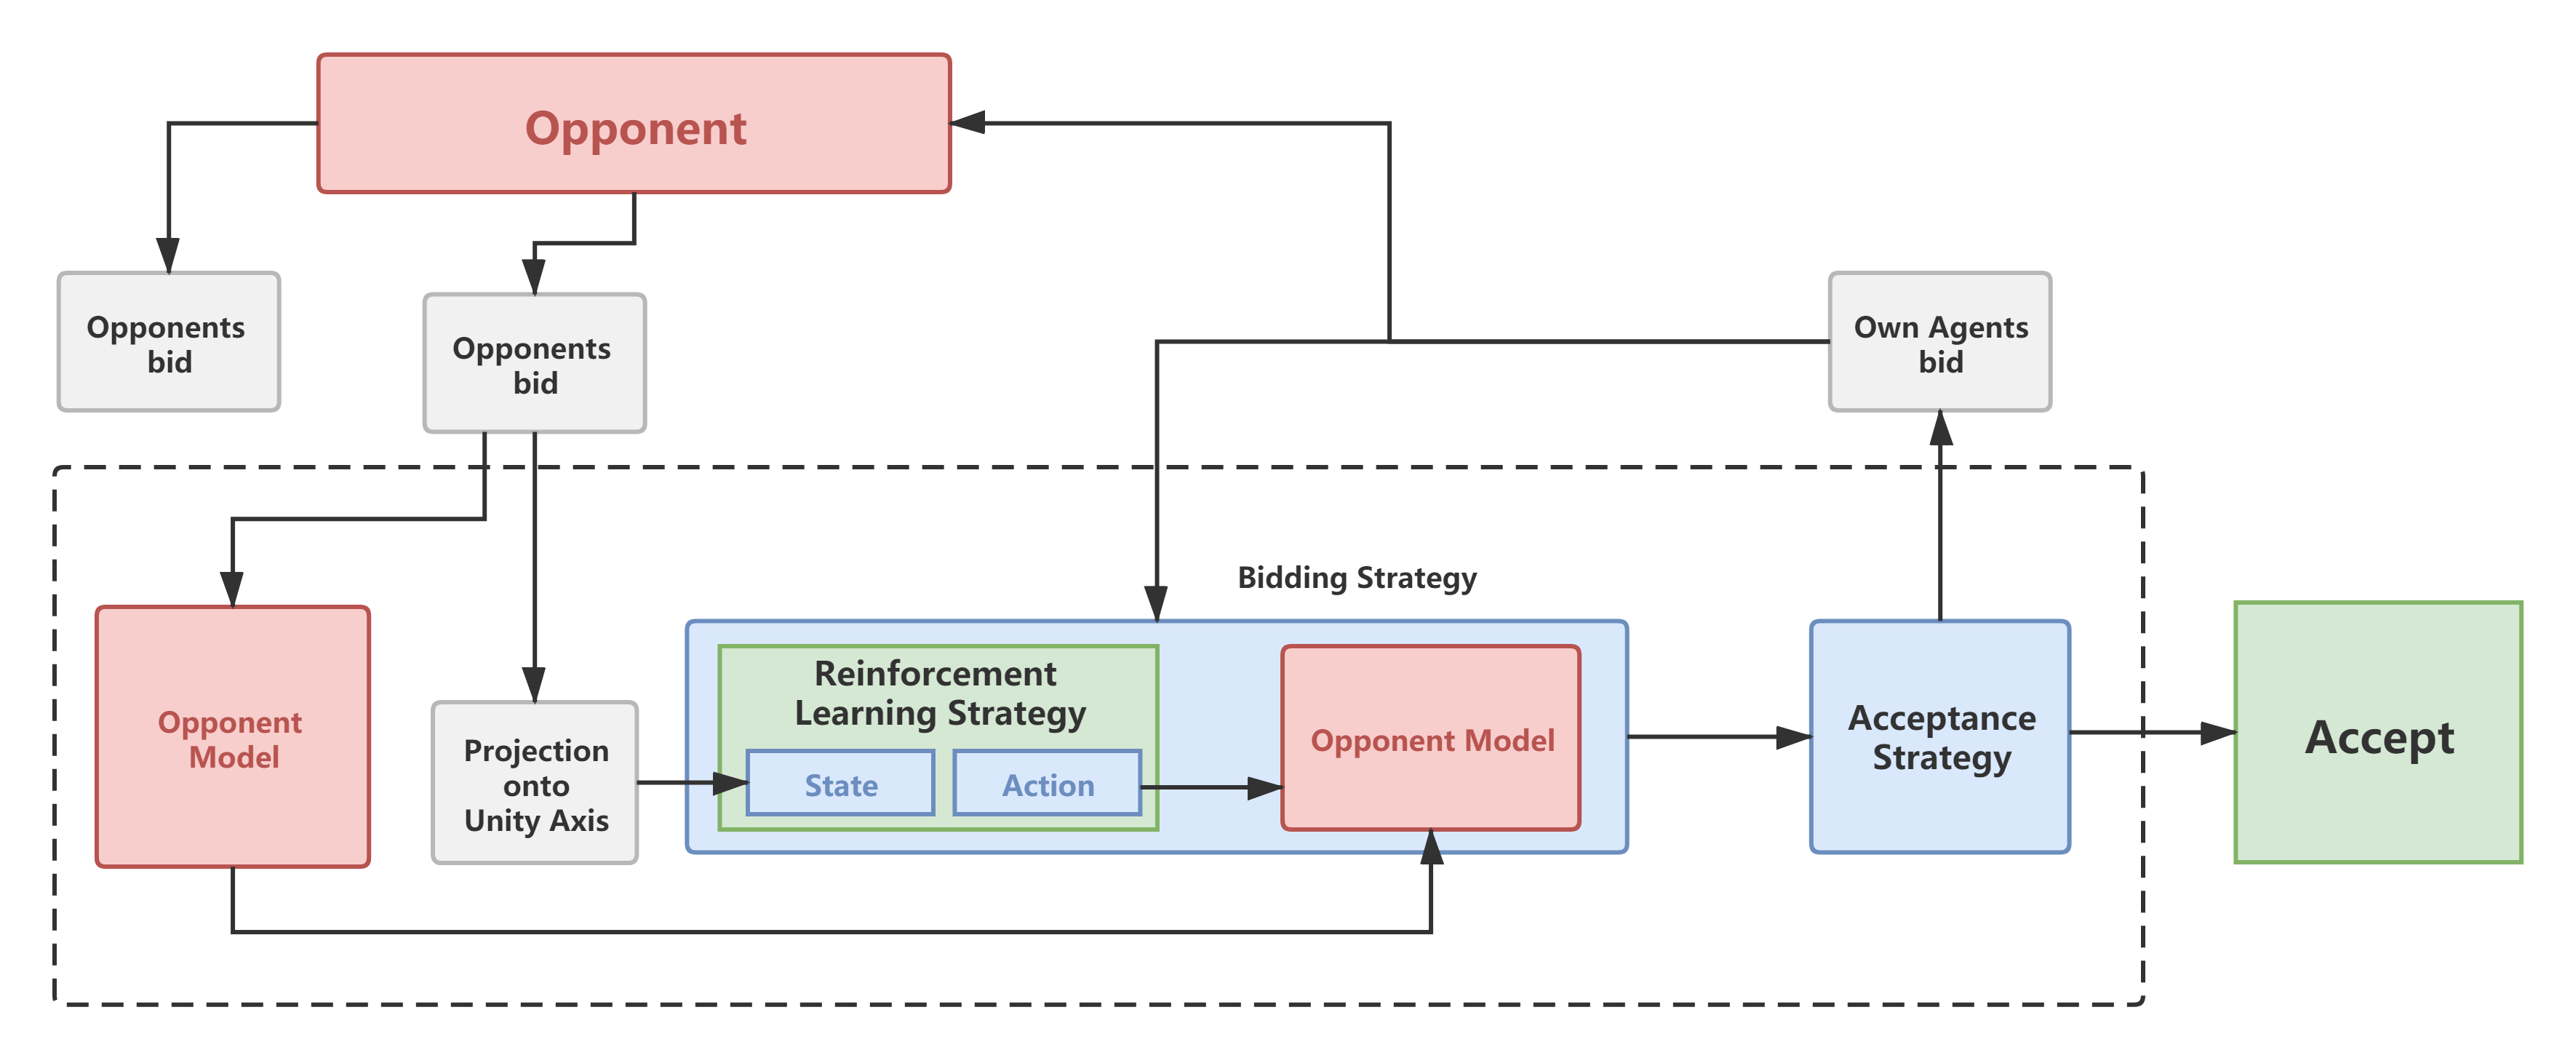
\includegraphics[width=1.0\textwidth]{./images/rlboa.png}
\caption{A schematic overview of the RLBOA-framework (within the dashed box), Source: Own illustration based
on\parencite{Bakker2019RLBOAAM}.}
\label{fig:rlboa}
\end{figure}


\paragraph{\gls{anegma}\parencite{bagga2020deep}:} Bag et. al. proposed a novel DRL-inspired agent model called ANEGMA, which allows the buyer to develop an adaptive strategy to effectively use against its opponents (which use fixed-but-unknown strategies) during concurrent negotiations in an environment with incomplete information. The architecture of \gls{anegma} is shown in Figure \ref{fig:anegma}. The agent uses an actor-critic architecture with model-free reinforcement learning. The method supervision from synthetic market data is adopted to pre-train the strategy. Especially, the proposed automated agents that can adapt to different settings without the need to be pre-programmed.

\begin{figure}[htbp]
\centering
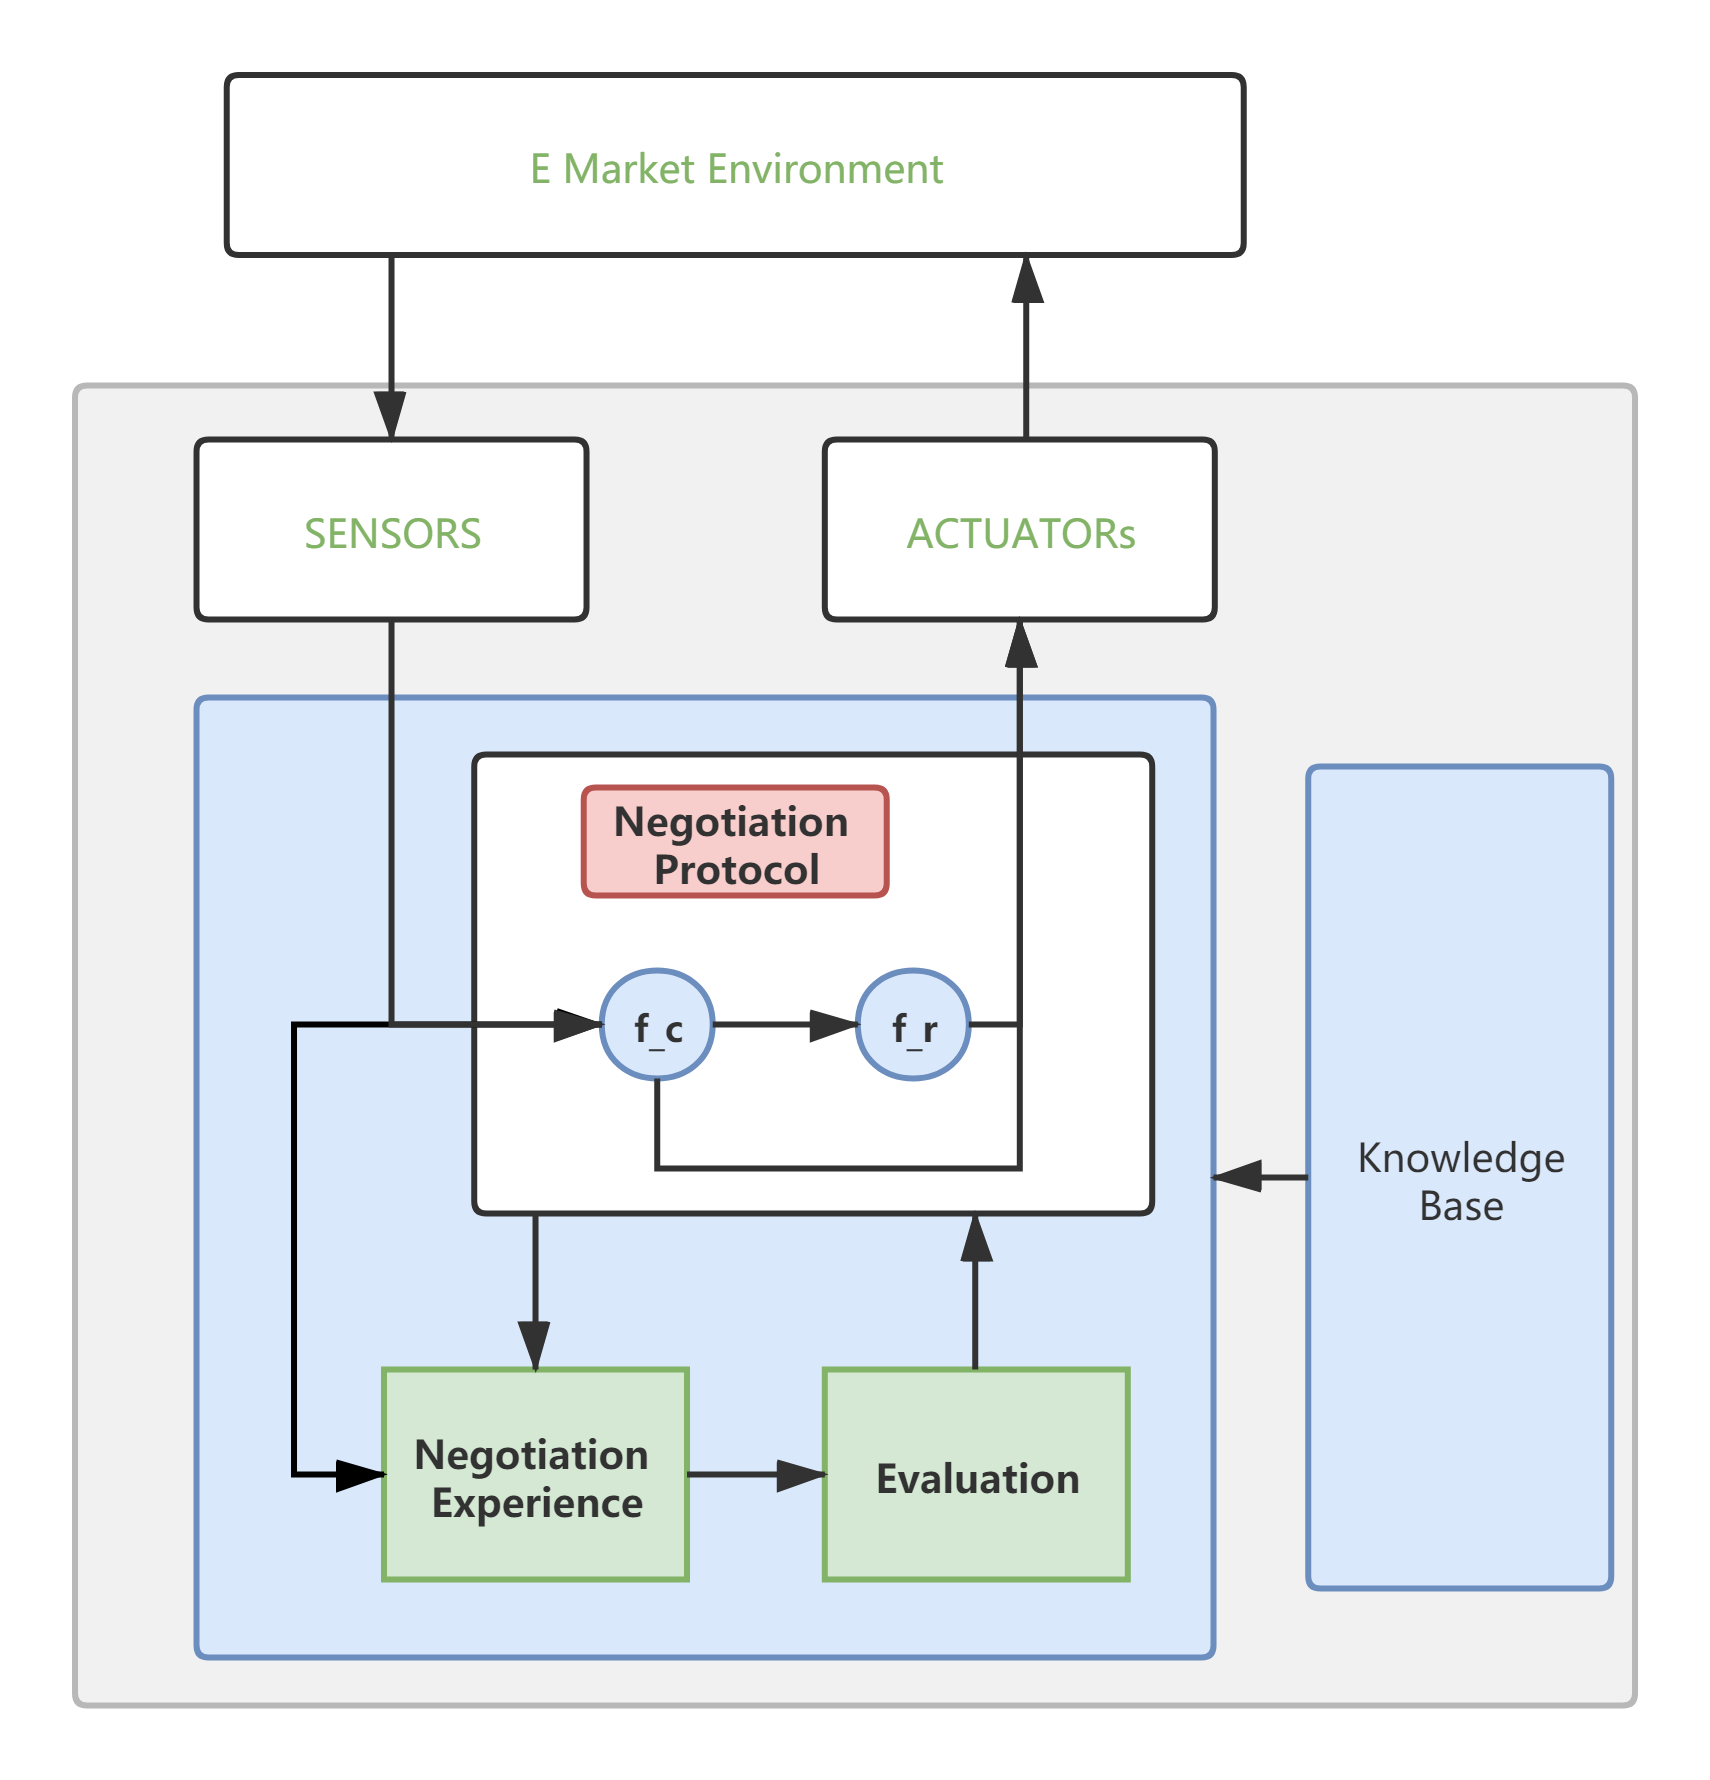
\includegraphics[width=0.8\textwidth]{./images/anegma.png}
\caption{The Architecture of \gls{anegma}. Source: Own illustration based on\parencite{bagga2020deep}.}
\label{fig:anegma}
\end{figure}

\subsection{Conclusion}
A lot of work has focused on the application of \gls{rl} in autonomous negotiation. The method of \textbf{decoupling strategy} can simplify the training process and make the behavior of the agent more clearly analyzed. The method \textbf{supervision from synthetic market data} is an impressive idea that can speed up the training of agents and reduce the exploration time required for learning during the negotiation process.

\section{Challenges in Deep Reinforcement Learning}

\subsection{Sparse Reward} \label{related-work:sparse-reward}
For financial problem, the reward is usually profit and an appropriate reinforcement learning signal should be based on it. However, when an agent learns the strategy just based on profit, the reward is too sparse. Hence, the reward function is needed to provide more frequent feedback. Methods \textbf{Reward Shaping},\textbf{ Curiosity Driven} and \textbf{Imitation Learning} proposed to solve sparse reward problem, will be introduced in this section.

\paragraph{Reward Shaping\parencite{Wiewiora2010}} is a method for engineering a reward function in order to provide more frequent feedback on appropriate behaviors. Providing feedback during early learning is crucial, so try promising behaviors as early as possible. This is necessary in large domains, where reinforcement signals may be few and far apart. If a method added shaping rewards in a way, it need to guarantees the optimal policy maintains its optimality. Ng et al. proposed a method with a new concept potential function $\Phi()$ to guarantee it. Hence, reward shpaing $f$ is described as $f(s, s^{\prime}) = \gamma\Phi(s^{\prime}) - \Phi(s)$ over the stats\parencite{Ng1999PolicyIU}. The form means shaping reward $f$ for transitioning from state $s^{\prime}$ to $s$ is defined as the discounted change in this state potential. Based on the value function mentioned in the section \ref{background:value-function}, the augmented value function is closely related to the original and is described as $V^{\prime}(s) = V(s) - \Phi(s)$. It is obvious to set potential function $\Phi(s) \approx V(s)$. This intuition is strengthened by results presented by Wiewiora in the paper \parencite{Wiewiora2003}.

 
\paragraph{Curiosity Driven \parencite{pathakICMl17curiosity}} The author designed a new intrinsic reward signal that describes the agent’s familiarity with the environment. The policy outputs a sequence of actions to maximize that intrinsic reward signal. In addition to intrinsic rewards, the agent optionally may also receive some extrinsic reward from the environment. Intrinsic rewards encourage agents to actively explore the environment, instead of staying in place due to lack of reward signals.

\paragraph{Imitation Learning\parencite{DBLP:journals/corr/HesterVPLSPSDOA17}} Inverse reinforcement learning (IRL) is a different approach of imitation learning, where the main idea is to learn the reward function of the environment based on the expert’s demonstrations, and then find the optimal policy.

\subsection{Non-stationary environment}
Traditional \gls{rl} research assumes that environment dynamical (i.e., \gls{mdp} parameters) are always fixed (i.e., stationary). However, this assumption is not realistic in many real-world environment. In \gls{scm} world, for instance, factories' can change their negotiation strategy during the simulation. The difficult question is how to deal with non-stationary rewards and non-stationary transition probabilities between system stats. Centralized training decentralized execution\parencite{maddpg2017} is a method for multi-agent learning under non-stationary environment. Besides, a method called \textbf{Context Q-learning}\parencite{Padakandla_2020} first detects the changes of environment with a detection algorithm. Using the results of the detection, this method can estimate the strategy of the new environment model, or if the environment model has been previously experienced, the learned strategy can be improved.

\subsection{Huge size of action space}
In many real-world environment, the tasks involve large numbers of discrete actions. Traditional \gls{rl} methods are difficult or even often impossible to apply to solve the problem. One proposed approach in the paper \parencite{dulacarnold2016deep} embed the large discrete actions in a continous space with prior information about the actions. Then, the action can be selected using approximate nearest-neighbor method. The lookup complexity is logarithmic-time relative to the number of actions.

Learning algorithms, which used to solve continuous action space do not need to calculate $Q$ value for every state-action pairs. It maintains just a policy $\pi$ and can output continuous action. One method is to replace the large discrete action space by continuous action space. Additionally, discrete actions can be determined based on the results.

\subsection{Conclusion}
There are many challenges in deep reinforcement learning. Although many solutions have been proposed, they are still difficult to apply, but they still have certain experimental significance. In this section, the work related to the three typical challenges helped understand and solve many of the problems in the work of this thesis. For example, in oder to solve the challenge of non-stationary environment, method centralised training decentralised execution is adapted in the training algorithm of multi-agent. For challenge of huge size of action space, one solution is that algorithms for continuous action space are used. For the design of the reward function, reward shaping helps to understand the shaping reward theoretically. This is a way to solve the sparse reward challenge. 